\begin{flushleft}

The L-system at its core is a formal grammar made up of an \textit{alphabet} of characters which are concatonated together into strings. The L-system describes a starting string of one or more characters called an \textit{axiom}. The L-system also describes a set of production rules, which determine whether a symbol in a string should be rewritten with another symbol or string. These rules are applied to each symbol in the \textit{axiom}. Once the production rules have been applied to the all of the symbols in the \textit{axiom} string, we may then use the resulting string as the new starting point, then iteratate over that string once again. This rewriting of strings, via the production rules is the mechanism for generating a structure of state transitions. Essentially the symbols represent a particular state of a system, and the production rules decide whether a state should transition based on a certain criteria, and if so, what the next state should be. \\

\vspace{5mm}

It is important to note that the L-system itself has no concept of what it is trying to represent, therefore, how the L-system is represented is left up to a separate system which is responsible for interpreting the resulting set of symbols in way that makes the most sense for that representation. For instance, the symbols for a L-system trying to represent a tree, may be interpreted very differently to the symbols trying to represent music, however, the L-system itself may be identical. \\
This chapter will discuss a number of different types of L-systems, as well as their features and limitations, whilst focusing on the mechanics behind the rewritting systems. I will then discuss the system which takes the resulting strings generated by the L-system, and interprets them in such a way that we can create 3D models of plant-life. \\

\vspace{5mm} 

A well-known biologist Aristid Lindenmayer, started work on the Lindenmayer System or L-system in 1968, he sought to create a new method of simulating growth in multicelular orgamisms such as algae and bacteria \cite{lindenmayer1968mathematical}. He later defined a formal grammar for simulating multicelular growth which he called the 0L-system \cite {lindenmayer1971developmental}. In the last twenty years, the concept has been adapted to be used to describe larger organisms such as plants and trees as well as other non organic structures like music \cite{worth2005growing}. There has also been studies to try and use an L-system as a method of creating and controlling growth of a connectionist model to represent human perception and cognision \cite{vaario1991connectionist}. More towards real human biology K{\'o}kai et al. (1999) have created a method of using a parametric L-system to describe the human retina, this can be combined with evolutionary operators and be applied to patients with diabetes who are being monitored \cite{kokai1999parametric}.

\end{flushleft}

\section{Simple DOL-system} \label{Simple DOL-systems}

\begin{flushleft}

According to Prusinkiewicz and Hanan a simple type of L-systems is known as a Deterministic 0L systems. It is deterministic as each symbol has an associated rule and there is no randomness in determining which rule should be chosen. The term '0L system' abbreviates 'Lindenmayer system with zero-sided interactions'. A zero-sided interactions refers to the multicellular representation of an L-system, where each symbol refers to a type of cell, and a 0L-system is a type of L-system that does not account for the state of its direct neighbouring symbols. There are three major parts to a D0L system. There is a finite set of symbols known as the (\textit{alphabet}), the starting string or (\textit{axiom}) and the state transition rules (\textit{rules}). The alphabet is a set of characters which represent a particular state in a system. The starting string or \textit{axiom} is the starting point of the system which contains one or more characters from the alphabet. The transition rules dictate whether a state should remain the same or transition into a different state or even disappear completely. \cite{prusinkiewicz2013lindenmayer}. \\

\vspace{5mm}

The DOL-system was originally created to serve as a context free grammar, which allows the multicellular organisms to be represented. In this case the each type of cell in represented in the L-system by a character in the alphabet, and the production rules represent the type of cell transitions that take place. In the DOL-system below, there is an example formulated by Prusinkiwicz and Lindenmayer to simulate Anabaena catenula which is a type of filamentous cyanobacteria which exists in plankton. According to Prusinkiewicz and Lindenmayer "Under a microscope, the filaments appear as a sequence of cylinders of various lengths, with $a$-type cells longer than $b$-type cells. And the subscript $l$ and $r$ indicate cell polarity, specifying the positions in which daughter cells of type $a$ and $b$ will be produced \cite{prusinkiewicz2012algorithmic}.

\vspace{5mm}

\begin{equation} \label{DOL-system example}
\begin{aligned}
	&\omega~~ : a_r \\
	&p_1~ :  a_r~ \rightarrow~ a_l b_r\\
	&p_2~ :  a_l~ \rightarrow~ b_l a_r\\
	&p_3~ :  b_r~ \rightarrow~ a_r\\
	&p_4~ :  b_l~ \rightarrow~ a_l\\
\end{aligned}
\end{equation}

\vspace{5mm}

With the deinition above, the DOL-system states $w~ :~ a_r$, $w$ signifies that what follows is the starting point (axiom), ergo, the starting point is the cell $a_r$. The production rules then follow and are $p1, p2, p3$ and $p4$. The : symbol separates the axiom and production names from their value, furthermore the $\rightarrow$ can be verbalised as "is relaced by" or "rewritten with". In production rule 1 ($p1$) the cell $a_r$ will be rewritten with cells $a_l b_r$, $p2$ states that $a_l$ will be rewritten with cells $b_l a_r$, $p3$ states $b_r$ will rewritten with cell $a_r$ and finally production rule 4 ($p4$), states that $b_l$ will be rewritten with cell $a_l$. In order to simulate Anabaena catenula we require these four rewritting rules, as there are four types of state transitions. \\

\vspace{5mm}

The resultant strings of five generations of the DOL-system rewritting process: \\

\vspace{5mm}

\begin{equation} \label{DOL-system result string}
\begin{aligned}
	& G_0~ :~ a_r \\
	& G_1~ :~ a_l b_r \\
	& G_2~ :~ b_l a_r a_r \\
	& G_3~ :~ a_l a_l b_r a_l b_r \\
	& G_4~ :~ b_l a_r b_l a_r a_r b_l a_r a_r \\
	& G_5~ :~ a_l a_l b_r a_l a_l b_r a_l b_r a_l a_l b_r a_l b_r \\
\end{aligned}
\end{equation}

\vspace{5mm}

During the rewriting process, generation zero ($G_0$) is the axiom. In subsequent generations the resultant string of the previous generation is taken and each symbol in the string is compared to the production rules, if they match a rule the symbol is rewritten with the next symbol or string that is specified by the production rule. For $G_1$ we take the previous generations resultant string which in this case is the resultant string of $G_0$, being $a_r$, the first symbol is compared with the production rule until it matches one. In this case it matches rule $p1$ with the rule $p1~ :~ a_r~ \rightarrow~ a_l b_r$ and therefore, $a_r$ is rewritten with $a_l b_r$. The $G_0$ resultant string only has one symbol it can be concluded that the resultant string of $G_1$ is $a_l b_r$. The resultant string of generation one is then rewritten to produce generation two and so on, untill we reach the desired number of generations.\\

\vspace{5mm}

\end{flushleft}

\section{Interpreting the DOL-system} \label{Interpreting DOL-system}

\begin{flushleft}

Section \ref{Simple DOL-systems} outlines a simple type of L-system known as the DOL-system, this L-system specifies a set of symbols, a starting point and a set of production rules, allowing us to represent a problem as a set of states. The prodcution rules can express valid state transisions, which thereafter allows us to produce a resulatant string of symbols that obay the L-systems production rules. This functionality is powerful in and of itself, however, the L-system's symbols are only usefull if they are capable of representing something meaningful in the real world, furthermore the L-system does not supply this meaning, each symbols meaning is interpreted after the rewriting process of the L-system. Due to this, there are two separate and very different systems involved in taking an L-systems input, such as the alphabet, axiom and production rules and turning it into something that is able to model plant-life. These two systems are the L-system rewriter is the system that is reposponsible for using the L-system definition in order to rewrite a string and provide a resultant string of symbols. The L-system interpreter takes the resultant string from the L-system rewriter and interprets in a way that is able to represent the model we are trying to create. \\

\vspace{5mm}

A paper by Przemyslaw Prusinkiewicz outlines a method for interpreting the L-system in a way that can model fractal structures, plants and trees. The method interprets the resultant string of the L-system, where each symbol represents an instructions which is carried out one after the other to control a 'turtle' \cite{prusinkiewicz1986graphical}. When talking about a turtle, prusinkiewicz is referring to turtle graphics. Turtle graphics is a type of vector graphics that can be carried out with instructions. It is named a turtle after one of the main features of the Logo programming language. The simple set of turtle instructions listed below, can be displayed as figure \ref{basic turtle}. The turtle starts at the base or root of the tree and interprets a set of rotation and translation movements, which when all executed one after the other, trace the points which make up the plant structure, when these points are then joined together the result is a fractal structure such as a plant or tree.\\

\vspace{5mm}

In the OL-system there are a number of symbols that represent a particular meaning to the L-system interpreter. Whenever the interpreter comes across one of these symbols in the resultant string, it is interpreted as a particular turtle instruction which can be seen in the table below:

\vspace{5mm}

\begin{table}[h!]
\begin{tabular}{ | c | l | }
\hline
	Instruction Symbol 	& Instruction Interpretation \\  
\hline
\hline
	F 					& Move forward by a specified distance whilst drawing a line\\
\hline
	f 					& Move forward by a specified distance without drawing a line\\
\hline
	+ 					& Yaw to the right specified angle.\\
\hline
	- 					& Yaw to the left by a specified angle.\\
\hline
	/ 					& Pitch up by specified angle. \\
\hline
	$\backslash$ 		& Pitch down by a specified angle.\\
\hline
	$\hat{}$ 			& Roll to the right specified angle.\\
\hline
	\& 					& Roll to the left by a specified angle.\\
\hline
\end{tabular}
\caption{Table of turtle instruction symbols and their meaning to the interpreter}
\label{instruction table 1}
\end{table}
\FloatBarrier


The turtle instructions are presented in such a way that allows movement in three dimensions, the rotations in yaw, pitch and roll are multiplied together, if the turtle moves forward again it will move in the direction of this new orientation. Diagram  \ref{3D rotations} shows the yaw, pitch and roll rotations and their associated interpretation names. \\ 

\begin{figure}[htbp]
	{\centering
		\setlength{\fboxrule}{1pt}
		\vspace{7px}
		\fbox{
			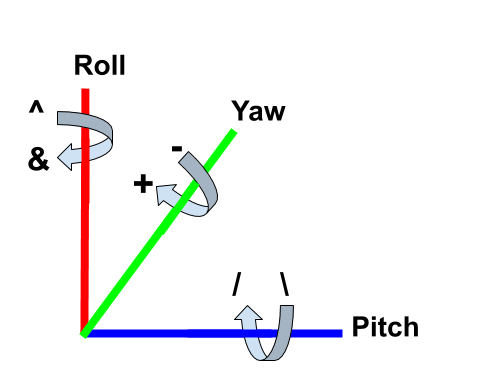
\includegraphics[scale=0.3]{Diagrams/rotations.png}
		}
		\caption{Diagram of the 3D rotations of the turtle.} \label{3D rotations}
	}
\end{figure}
\FloatBarrier

\vspace{5mm}

The turtle instructions in the table \ref{instruction table 1}, can be used as the alphabet for the rewriting system in the the L-system grammar below:

\begin{equation} \label{DOL-system example}
\begin{aligned}
	&\text{Generations: 1}\\
	&\text{Angle: 90$^{\circ}$}\\
	&\omega~~ : F \\
	&p_1~ :  a_r~ \rightarrow~ F+F-F-F+F\\
\end{aligned}
\end{equation}

\vspace{5mm}

With the L-system above the resulting string would be "F+F-F-F+F", this string can be interpreted using turtle graphics to give a list of instructions.

\vspace{5mm}

Instruction 1. Move forward by 1.\\
Instruction 2. Rotate right by 90 degrees.\\
Instruction 3. Move forward by 1.\\
Instruction 4. Rotate left by 90 degrees \\
Instruction 5. Move forward by 1. \\
Instruction 6. Rotate left by 90 degrees. \\
Instruction 7. Move forward by 1. \\
Instruction 8. Rotate right by 90 degrees. \\
Instruction 9. Move forward by 1.\\

\vspace{5mm}

talk about the complexities of each system. 

\vspace{5mm}

\begin{figure}[htbp]
	{\centering
		\setlength{\fboxrule}{1pt}
		\vspace{7px}
		\fbox{
			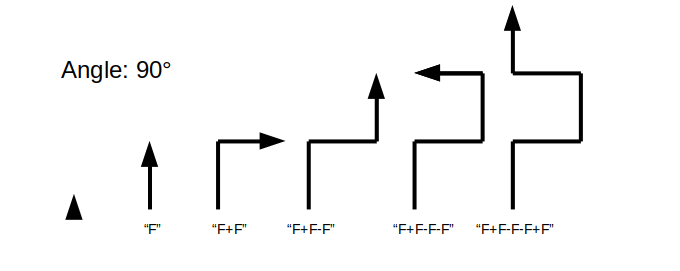
\includegraphics[scale=0.5]{Diagrams/basic_turtle.png}
		}
		\caption{Diagram showing a turtle interpreting simple L-system string.} \label{basic turtle}
	}
\end{figure}
\FloatBarrier

\vspace{5mm}

There are a further two commands which I will be covering in detail in section \ref{branching}. We can also have constant numerical values that can be used. For instance, we could pass in a constant value of 1.0 as a parameter to the forward instruction as follows.

\vspace{5mm}

F(1.0)+F(1.0)-F(1.0)+F(1.0)

\vspace{5mm}

In doing this, we can specify that we would like to move forward by a specified amount. In this case we would like to move forward by 1.0 unit length. We will be covering parametric L-systems in detail in section \ref{parametric}.

\end{flushleft}

\section{Branching} \label{branching}

\begin{flushleft}

In the previous section there are two turtle commands in particular which were  not covered. These are the square bracket commands '[', ']'. The square bracket characters instruct the turtle object to save its position and rotation for the purpose of being able to restore that saved position and rotation later on. This allows the turtle to jump back to a previous position, facing the same direction as it was before. We can then branch off in a different direction.\\

\vspace{5mm}

A way to keep track of these saved locations, is in the form of a stack structure. Each time the '[' is called the current position and orientation of the turtle is saved to the top of the stack. While conversely when the ']' is called we restore the turtles position back to whatever position and orientation is stored on the top of the stack. \\

\vspace{5mm}

An example of this can be shown below in figure 2.2.\\

\begin{figure}[htbp]
	{\centering
		\setlength{\fboxrule}{1pt}
		\vspace{7px}
		\fbox{
			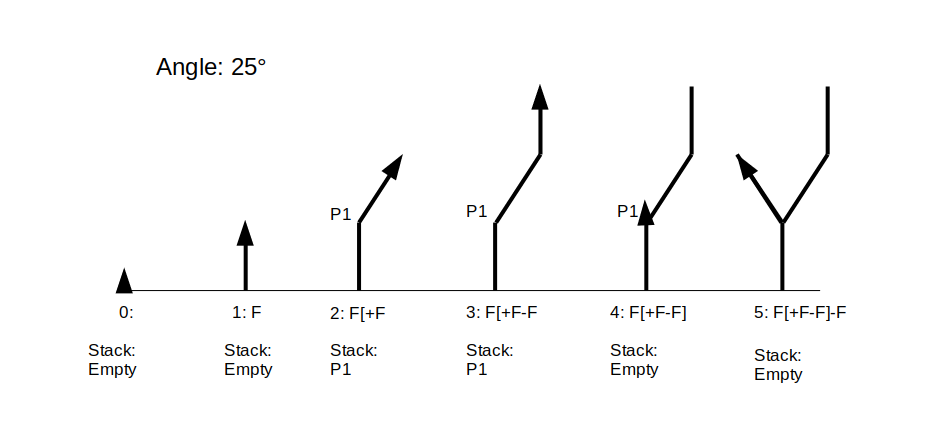
\includegraphics[scale=0.35]{Diagrams/branching_turtle.png}
		}
		\caption{Diagram showing a turtle interpreting an L-system incorporating branching.}
	}
\end{figure}
\FloatBarrier

\end{flushleft}

\section{Parametric OL-system} \label{parametric}

\begin{flushleft}

Simplistic L-systems like the algae representation in section \ref{Simple DOL-systems} above, give us enough information to create a very basic structure of plant life, there are many details that are not included which a simple OL-system will not be able to represent. With the simplistic approach we have assumed that the width and length and branching angles of each section is constant or predefined. The result of this was that all of the details such as width and length of branchesis left up to the interpretation of the resultant L-system string. This begs the question as to how we should accurately interpret the L-system string when we are not provided the details by the L-system. The answer lies in parametric 0L-systems.

\vspace{5mm}

In this section I will outline the definition and major concepts of the parametric L-system formulated by Prusinkiewicz and Hanan in 1990 \cite{prusinkiewicz1990visualization}, and developed upon in 2012 by Prusinkiewicz and Lindenmayer \cite{prusinkiewicz2012algorithmic}. I will also be talking about some of the changes that I have made, and explaining why these changes are necessary for the purpose of this thesis.

\end{flushleft}

\subsection{Definition of a Parametric 0L-system}

\begin{flushleft}

Prusinkiewicz and Hanan define the parametric 0L-systems as a system of parametric words, where a string of letters make up a module name $A$, each module has a number of parameters associated with it. The module names belong an alphabet $V$, therefore, $A~ \in~ V$, and the parameters belong to a set of real numbers $\Re$. If $(a_1,~ a_2,~ ...,~ a_n)~ \in~ R$ are parameters of $A$, the module can be stated as $A(a_1,~ a_2,~ ...,~ a_n)$. Each module is an element of the set of modules $M~ =~ V~ \times~ \Re^*$. $\Re^*$ represents the set of all finite sequences of parameters, including the case where there are no parameters. We can then infer that $M^*~ =~ (V~ \times~ \Re^*)^*$ where $M^*$ is the set of all finite modules. \\
Each parameter of a given module corresponds to a formal definition of that parameter defined within the L-system productions. Let the formal definition of a parameter be $\Sigma$. $ E(\Sigma) $ can be said to be an arithmetic expression of a given parameter.\\ Similar to the arithmetic expressions in the programming languages C/C++, we can make use of the arithmetic operators $ +,~ -,~ *,~ \,~ \wedge{}$. Furthermore, we can have the relational expression $C(\Sigma)$, with a set of relational operators. In the literature by Prusinkiewicz and Hanan the set of relational operators is said to be $<,~ >,~ =$, I have extended this to include the relational operators $>,~ <,~ >=,~ <=,~ ==,~ !=$. Where $==$ is the 'equal to' operator and $!=$ is the 'not equal' operator, and the symbols $>=$ and $<=$ are 'greater than or equal to' and 'less than or equal to' respectively. The parentheses () are also used in order to specify precedence within an expression. The arithmetic expressions can be evaluated and will result in the real number parameter $\Re $, and the relational expressions can be evaluated to either true or false. \\

\vspace{5mm}

The parametric 0L-system can be shown as follows as per Prusinkiewicz and Hanan's definition:\\

\vspace{5mm}

\begin{equation}
G~ = (V, \Sigma, \omega, P)
\end{equation}
\vspace{5mm}

$G$ is an ordererd quadruplet that describes the parametric OL-system. $V$ is the alphabet of characters for the system. $\Sigma$ is the set of formal parameters for the system. $\omega~ \in~ (V~ \times \Re^*)^+$ is a non-empty parametric word called the axiom. Finally $P$ is a finite set of production rules which can be fully defined as:

\vspace{5mm}

\begin{equation}
P~ \subset~ (V~ \times~ \Sigma^*)~ \times C(\Sigma)~ \times~ (V~ \times~ E(\Sigma))^*
\end{equation}

\vspace{5mm} 

Where $(V~ \times~ \Sigma^*) $ is the predecessor module, $C(\Sigma) $ is the condition and $(V~ \times~ E(\Sigma))^* $ is the set of successor modules. For the sake of readability we can write out a production rule as \textit{predecessor} : \textit{condition} $\rightarrow$ \textit{successor}. I will be explaining the use of conditions in production rules in more detail in section \ref{Condition L-system Subsection}.\\
A module is said to match a production rule predecessor if they meet the three criteria below. In the case where the module does not match any of the production rule predecessors, the module is left unchanged, effectively rewriting itself. \\

\vspace{5mm}

$\bullet$ The name of the axiom module matches the name of the production predecessor. \\
$\bullet$ The number of parameters for the axiom module is the same as the number of parameters for the production predecessor. \\
$\bullet$ The condition of the production evaluates to true. If there is no condition, then the result is true by default.\\

\vspace{5mm}

\end{flushleft}

\subsection{Defining Constants and Objects}

There are some other features covered by Prusinkiewicz and Lindenmayer, that are not specific to the parametric L-systems definition itself but serve more as quality of life. In the literature, they refer to the \#define which is said "To assign values to numerical constants used in the L-system" as well as the \#include statement which specifies what type of shape to draw by refering to a library of predefined shapes \cite{prusinkiewicz2012algorithmic}. \\
For instance if we have an value for an angle that we would like to use within the production rules we can use the \#define statement as follows:

\vspace{5mm}

\begin{equation} \label{define statement example}
\begin{aligned}
	&n=4 \\
	&\textrm{\#define angle 90}\\
	&\omega~~ : F(5)\\
	&p_1~ :  F(x)~~~~~ :~ * \rightarrow~ F(w)+(angle)F(w)+(angle)F(w)+(angle)F(w)\\
\end{aligned}
\end{equation}

\vspace{5mm}

Here you can see that the \#define acts like a declaration, where we are going to be defining a variable which will be used later. Essentially we are replacing any occurences of the variable \textit{angle} with the value of 90 degrees. The define statement is written as  \#define \textit{variable\_name} \textit{value}. \\

\vspace{5mm}

With regards to the \#include statement, In the literature the \#include may be used by stating '\#include H'. This would tell the turtle interpreter that the symbol 'H' is a shape in a library of predefined shapes which should be rendered instead of the default shape. We have decided modify this functionality, instead of the \#include statement, we have provided the \#object statement. The \#object statement serves a similar purpose however instead of import the symbol 'H' we can specify, \#object H HETEROCYST, which specifies that we are associating the symbol or module 'H' with the object HETEROCYST. The HETEROCYST object will be stored in a predefined library. This way we can associate the same object to multiple symbols. It also does not limit us to a predefined name for an object. Below is an example using the \#object statement: \\

\vspace{5mm}

\begin{equation} \label{object statement example}
\begin{aligned}
	&n=1 \\
	&\textrm{\#object F BRANCH}\\
	&\textrm{\#object S SPHERE}\\
	&\omega~~ : F(1)\\
	&p_1~ :  F(x)~~~~~ :~ * \rightarrow~ F(w)F(w)F(w)F(w)S(w)\\
\end{aligned}
\end{equation}

\begin{figure}[htbp]
	{\centering
		\vspace{7px}
		\setlength{\fboxrule}{1pt}
		\fbox{
			
\includegraphics[scale=0.2]{Diagrams/object_example.png}
		}
		\caption{Diagram of an L-system Using Multiple Objects.}
	}
\end{figure}
\FloatBarrier

\vspace{5mm}

In the simple example in figure \ref{object statement example} above, you can see that the first three F modules render a branch segment with length of 1.0, however for the final module the S module renders a sphere of diameter 1.0. It is possible  

I will be going into more detail about this and other features in section \ref{l-system generator section}.

\subsection{Modules With Special Meanings}

\begin{flushleft}


In the above section I defined the details of a parametric 0L-system, in the paper by Prusinkiewicz and Lindenmayer, there are two operators which I have not discussed yet, those are the ! and the ‘. Prusinkiewicz and Lindenmayer state that “The symbols ! and ‘ are used to decrement the diameter of segments and increment the current index to the color table respectively” \cite{prusinkiewicz2012algorithmic}. We have decided to modify this to work slightly differently, the ! and ‘ will still perform the same operation, however the ! and ‘ symbols are actually treated as a module that holds a particular meaning to the interpreter, rather than a single operator, furthermore, they share the same properties with modules, they can contain multiple parameters, and depending on the number of parameters they can be treated differently. The module ! with no parameters could mean decrement the diameter of the segment by a default amount, whereas !(10) means set the diameter of the segment to 10. The length can also be manipulated in a similar manner. The module with the name F has a default meaning to create a segment in the current direction by a default amount. If we provide the module F(10) we are specifying to create a segment of length 10.\\

\vspace{5mm}

Using the L-system below we can create figure \ref{parametric l-system practical}, the concepts discussed above have been used by decrementing the segment diameter during the rewriting process as well as by incrementing the branch length.

\vspace{5mm}

\begin{equation} \label{parametric l-system practical}
\begin{aligned}
	&n=8 \\
	&\omega~~ : A(5)\\
	&p_1~ :  A(w)~~~~~ :~ * \rightarrow~ F(1)!(w)[+A(w~*~0.707)][-A(w~*~0.707)]\\
	&p_2~ :  F(s)~~~~~ :~ * \rightarrow~ F(s~*~1.456)\\
\end{aligned}
\end{equation}

\vspace{5mm}

The above l-system gives the resulting representation shown below in figure 3.8. 

\begin{figure}[htbp]
	{\centering
		\vspace{7px}
		\setlength{\fboxrule}{1pt}
		\fbox{
			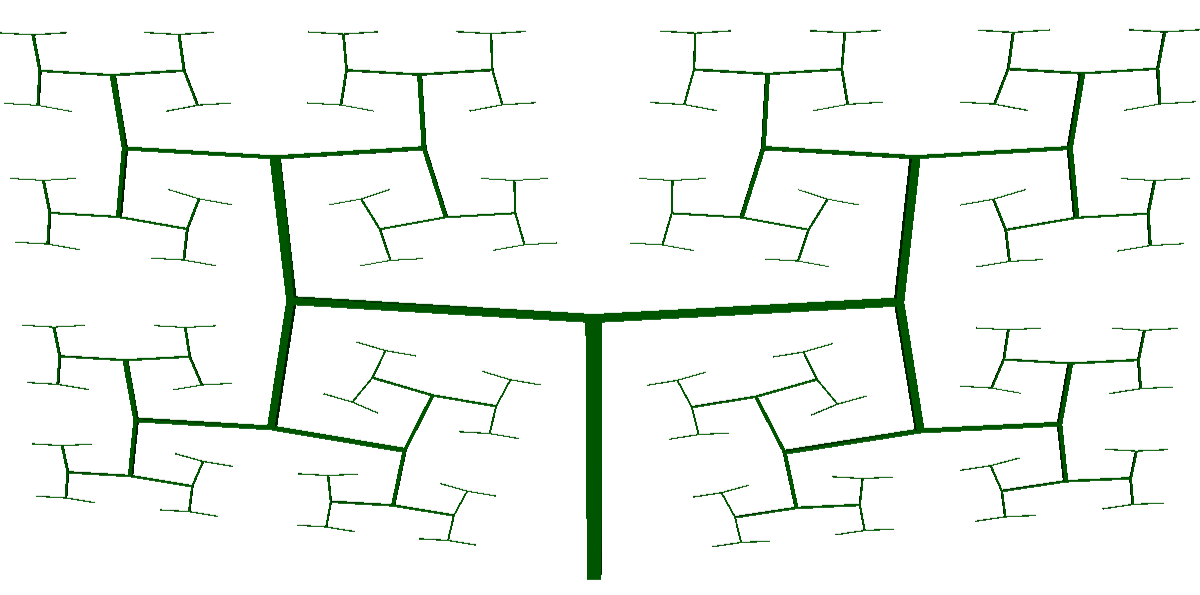
\includegraphics[scale=0.20]{ParametricLsystem/branchingPattern.png}
		}
		\caption{3D Parametric L-system.}
	}
\end{figure}

\FloatBarrier

This gives a much more realistic looking tree structure as the branch segments become shorter but also become thinner in diameter as they get closer to the end of the branch as a whole. 

\end{flushleft}



\subsection{Representing L-system Conditions} \label{Condition L-system Subsection}

\begin{flushleft}

A condition allows us to have multiple production rules that are the same in terms of the module name and the number of parameters that they have, furthermore, they require a particalar condition to be met in order for the module to match that rule. \\
In this section I will be detailing the use of the condition statement, which lies between the predecessor and the successor in a production rule, and can be seen as an a mathematical expression on either side of a relational operator. During the rule selection process the expressions are evaluated and the results are compared using the condition operator. If the result of the condition is true then that rule is selected for rewriting, if the result is false then it moves on to check the next rule. \\

\vspace{5mm}

Below is an example of a parametric 0L-system using condition statements:\\

\begin{equation} \label{parametric l-system example}
\begin{aligned}
	&n=5 \\
	&\omega~~ : A(0)B(0,4)\\
	&p_1~ :  A(x)~~~~~ :~ x~ >~ 2~ \rightarrow~ C\\
	&p_2~ :  A(x)~~~~~ :~ x~ <~ 2~ \rightarrow~ A(x~ +~ 1)\\
	&p_3~ :  B(x,~ y)~ :~ x~ >~ y~ \rightarrow~ D\\
	&p_4~ :  B(x,~ y)~ :~ x~ <~ y~ \rightarrow~ B(x~ +~ 1,~ y)\\
\end{aligned}
\end{equation}

\vspace{5mm}

The L-system above in \ref{parametric l-system example} is rewritten five times using the axiom specified by the symbol $\omega$, as well as the four production rules $p_1, p_2, p_3, p_4$. Each generation of the rewritting process can be seen below in \ref{parametric l-system example result}.

\vspace{5mm}

\begin{equation} \label{parametric l-system example result}
\begin{aligned}
	&g_0 :~ A(0)B(0,~4)\\
	&g_1 :~ A(1)B(1,~4)\\
	&g_2 :~ A(2)B(2,~4)\\
	&g_3 :~ C~B(3,~4)\\
	&g_4 :~ C~B(4,~4)\\
	&g_5 :~ C~D\\
\end{aligned}
\end{equation}

\vspace{5mm}

A practical use of the condition statement might be to simulate different stages of growth. This is best illustrated using the L-system below: \\

\vspace{5mm}

\begin{figure}[htbp]

\begin{equation} \label{conditional l-system example}
\begin{aligned}
	&n=2,~4,~6 \\
	&\#\text{object F BRANCH} \\
 	&\#\text{object L LEAF} \\
	&\#\text{object S SPHERE} \\
	&\#\text{define r 45} \\
	&\#\text{define len 0.5} \\
	&\#\text{define lean 5.0} \\
	&\#\text{define flowerW 1.0} \\
	&\omega~~ :~ !(0.1)I(5)\\
	&p_1~ :  I(x)~ :~ x~ >~ 0~~ \rightarrow~ F(len)-(lean)[R({0, 100})]F(len)[R({0, 100})]I(x-1)\\
	&p_2~ :  R(x)~ :~ x~ >~ 50~ \rightarrow~ -(r)/(20)!(2.0)L(2)!(0.1)\\
	&p_3~ :  R(x)~ :~ x~ <~ 50~ \rightarrow~ -(r)\backslash(170)!(2.0)L(2)!(0.1)\\
	&p_4~ :  I(x)~ :~ x~ <=~ 0~ \rightarrow~ F(len)!(flowerW)S(0.3)\\
\end{aligned}
\end{equation}

	{\centering
		\vspace{7px}
		\setlength{\fboxrule}{1pt}
		\fbox{
			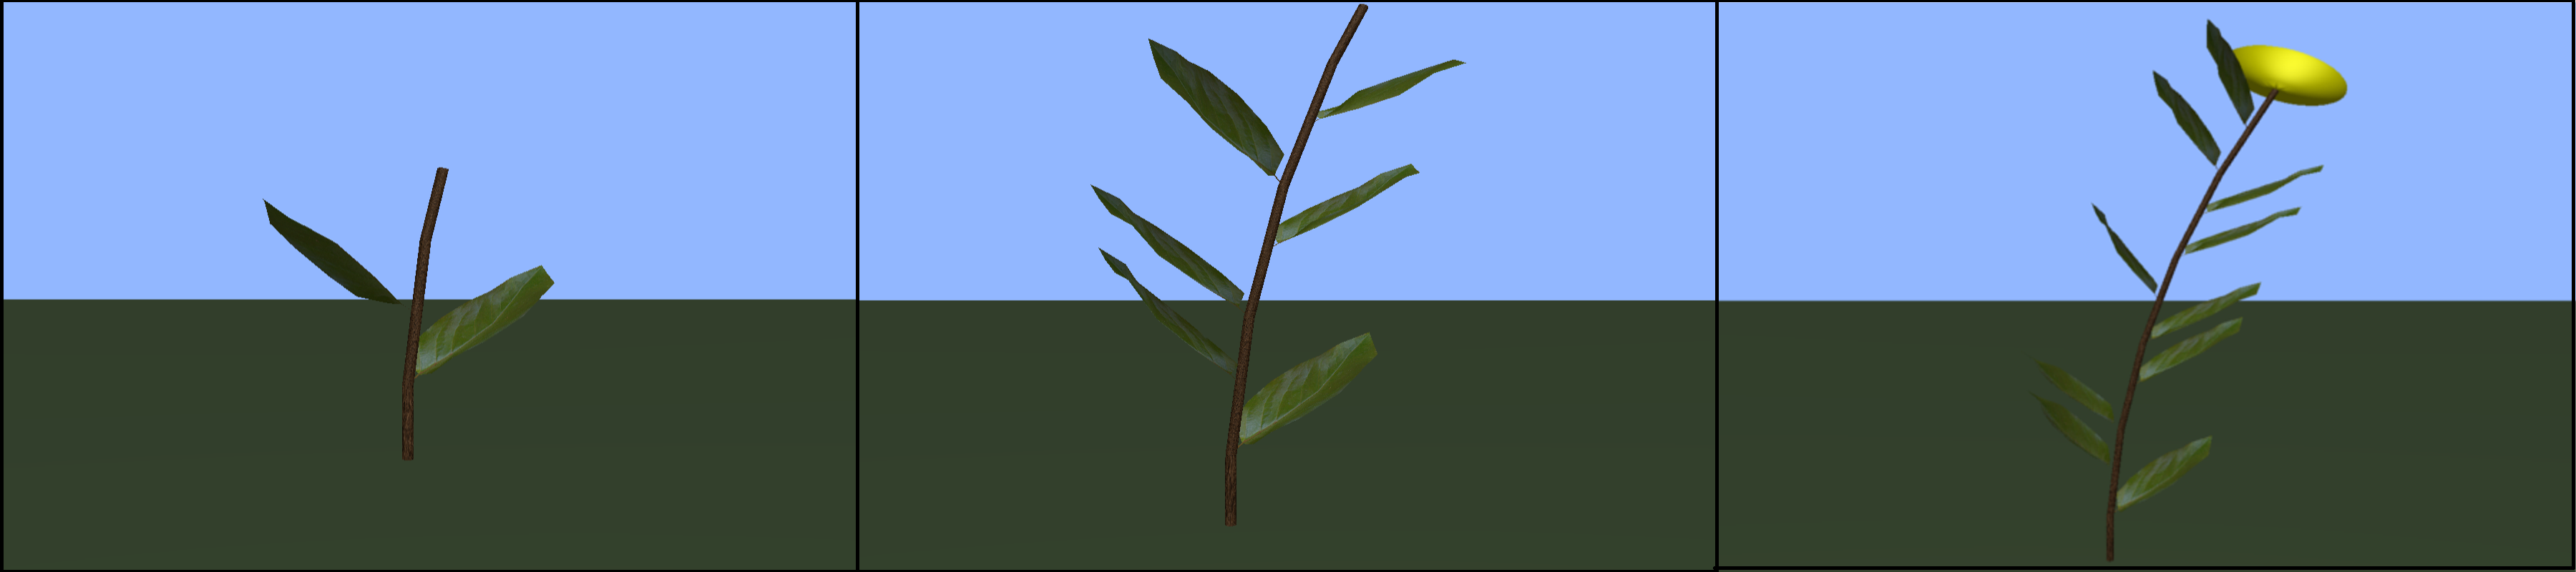
\includegraphics[scale=0.13]{Diagrams/conditionalLsystem.png}
		}
		\caption{Condition Statements Used to Simulate the Growth of a Flower. 2nd Generation on the Left, 4th Generation in the Center and 6th Generation on the Right}
	}
\end{figure}

\FloatBarrier

\end{flushleft}


\subsection{Representing Randomness} \label{Randomness L-system Subsection}

\begin{flushleft}

Randomness is an essential part of nature. If there was no randomness in plant life, we would end up with very symetric and unrealistic plants. Randomness is also responsible for creating variation in the same L-system. A L-system essentially describes the structure and species of a plant. It describes everything from how large the trunk of the tree is, to how many leaves there are on the end of branch, or even if it has flowers or not. However if there is no capability to have randomness in the generation of the L-system then we will always end up with the exact same structure. 
\vspace{5mm}
Below is a simple example of how randomness can be used to create variation.

\end{flushleft}   

\begin{figure}[htbp]
	\raggedright
	\textbf{\underline{Random Fractal:}} \\
	\#n = 2; \\
	\#w : !(0.2)F(1.0); \\
	\#p1 : F(x) : * : F(x)[+(25)F(x)][-(25)F(x)]+(\{-20.0, 20.0\})F(x)-(\{-20.0, 20.0\})F(x);\\
	\vspace{10mm}
	{\centering
		\vspace{7px}
		\setlength{\fboxrule}{1pt}
		\fbox{
			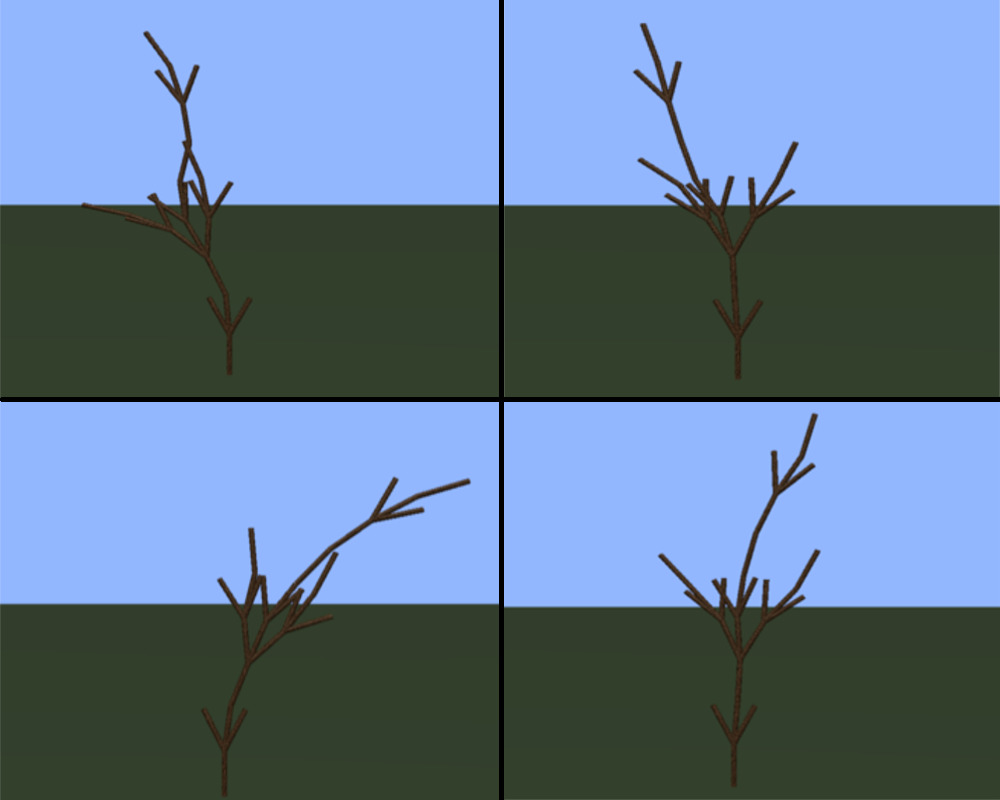
\includegraphics[scale=0.20]{Diagrams/RandomTrees.png}
		}
		\caption{Different Variations of the Same L-system with Randomness Introduced in The Angles. \label{figRandomness}}
	}
\end{figure}
\FloatBarrier

\begin{flushleft}

In figure \ref{figRandomness} there are four variations of the same L-system using randomness, We can specify that we would like to create a random number by using the expression \{-20.0, 20.0\}. The curly braces signify that what is contained is a random number range, ranging from the minimum value as the first floating point value and the maximum value as the second floating point value separated by a comma. If both values are the same for instance +(\{10.0, 10.0\}) this is equivilant to +(10.0).

\end{flushleft}

\subsection{Stochastic Rules in the L-system} \label{Stochastic L-system Subsection}

\begin{flushleft}

\begin{figure}[htbp]
	{\centering
		\vspace{7px}
		\setlength{\fboxrule}{1pt}
		\fbox{
			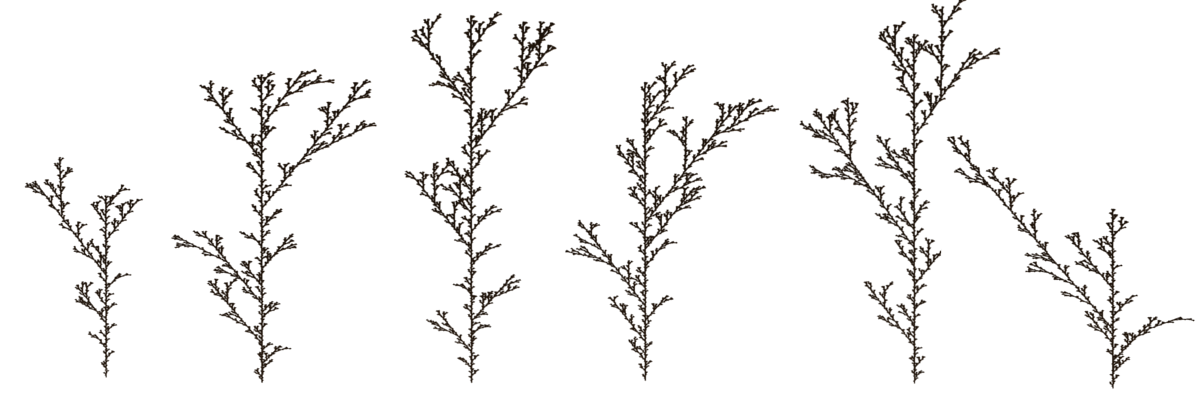
\includegraphics[scale=0.35]{Diagrams/stochastics.png}
		}
		\caption{Representation of an L-system with a probability stochastic with a 33.33\% chance for each rule.}
	}
\end{figure}

\FloatBarrier


\end{flushleft}






